\section{Theory}
\subsection{Neural Network Quantum State}
The Neural Network Quantum State (NQS) For this project, as mentioned, 
Instead of going with the approach of finding a trial wave function for the system, as done in our previous project, we are going to represent the state by a Neural Network Quantum State using the Restricted Boltzman Machine (RBM) as our as our Neural Network (NN) of choice. This approach of representing the wavefunction with a RBM was first done recently by G. Carleo and M. Troyer in 2017 [\textcolor{blue}{Solving the quantum many-body problem with artificial neural networks}]. However, in their project, they .... while we

\subsection{The System}
We will be considering a system of electrons, confined in a pure two-dimensional 
isotropic harmonic oscillator potential with an idealized total Hamiltonian which is given by,
%[We will simulate two electrones trapped in a HO trap]
\begin{equation}
\label{eq:finalH}
\hat{H}=\sum_{i=1}^{N} \left(  -\frac{1}{2} \nabla_i^2 + \frac{1}{2} \omega^2r_i^2  \right)+\sum_{i<j}\frac{1}{r_{ij}},
\end{equation}
where we are using the natural units given by ($\hbar=c=e=m_e=1$) and all the energies are given in atomic units (a.u). The first term of our Hamiltonian represents the the \textit{kinetic $+$ potential} energy. This part includes the standard harmonic oscillator part, which we call $\hat{H}_0$, where $N$ is the number of electrons as functions of the oscillator frequency $\omega$.\\ While the last term comes from the columb interaction given by
\begin{equation*}
\hat{H}_1 = \sum_{i<j}\frac{1}{r_{ij}} = \sum_{i=1}^{X-1} \sum_{j=i+1}^{X} \frac{1}{|\mathbf{r}_i - \mathbf{r}_j|}
\end{equation*}
where $r_{ij} = \abs{\mathbf{r}_i - \mathbf{r}_j}$ is the distance between two electrons, where the modulus of the positions of the electrons (for a given electron $i$) is $r_i = \sqrt{r^2_{i_x} + r^2_{i_y}}$. \\

For a one dimensional harmonic oscillator, the Energy is given by
\begin{equation*}
    E_n = \hbar \omega (n + \frac{1}{2}).
\end{equation*}
For our project, we will use $\hbar \omega = 1$, which means that the ground state energy for the 1D harmonic oscillator is $E_0  = \frac{1}{2}$ a.u. For the corresponding two dimensional harmonic oscillator with the interaction of electrons included, the ground state energy is $E_0 = 3$ a.u, and $2$ a.u for our unperturbed part $H_0$  [\textcolor{blue}{M.Taut 1993}] \\
Further, spacial part of the Wave function for the two dimensional harmonic oscillator with one electron, ignoring the the Columb interaction, is given by, \begin{equation*}
\phi_{n_x,n_y}(x,y) = A H_{n_x}(\sqrt{\omega}x)H_{n_y}(\sqrt{\omega}y)\exp{(-\omega(x^2+y^2)/2)}.
\end{equation*}
where A is our normalization constant and $H_{n}(\sqrt{\omega}y)$ are the Hermite polynomials. The ground state energy, i.e $n_x=n_y = 0$, we get the expression
\begin{equation*}
    \phi_{0,0} = A\exp{(-\omega(x^2+y^2)/2)},
\end{equation*}
which is the ground state for the unperturbed Wave function for the two-electron system. Further, from the above, we get that the energy eigenvalue is given by,  $$\epsilon_{n_x,n_y}=\omega(n_x+n_y+1) = \omega$$. \\
\subsection{Neural Networks}
Artificial Neural Networks, or simply just Neural Networks (NN), are computer systems which are modeled after the biological neural networks of animal brains. Just like biological brains, Neural Networks consists of neurons which either activate or or not depending on if a given threshold is reached. Each connection of a Neural Network can be compared with the synapses of a biological brain. They transmit signals to other neurons. However, biological neural networks learn through a process called synaptic plasticity, while artificial while learn by adjusting it's weights and biases in order to minimize a given cost function. The weights of the Neural Network are the connections between two neurons. In Graph Theory, we would refer to them as (weighted) edges between nodes. (while the bias is....). 
\\
A Neural Network consists of an input layer, a hidden layer, or multiple hidden layers as in the case of deep neural networks, and an output layer. [\textcolor{blue}{Figure 1}]

\begin{figure}[htbp]
  \centering
  \includesvg[scale= 0.4]{Neural-Network.svg}
  \caption{A simple Feed-forward Neural Network with 3 input neurons, 1 output neuron and 3 layers of hidden layers consisting of 4 neurons each.}
\end{figure}

(Write a little bit about the difference between supervised and unsupervised learning)

\subsection{The Restricted Boltzmann Machine}
For our Neural Network of choice, we will be implementing the Restricted Boltzmann Machine. The RBM is a Markov Random Field witch consists of a visible layer and a hidden layer where both the layers are stochastic. We will call the set of visible neurons for $\mathbf{X}$ and our set of hidden neurons for $\mathbf{H}$. Since it's restricted, there is no connection between two nodes of the same layer. In other words, there is only a connection between two nodes if one is visible whilst the other is hidden. Further, the RBM is a Generative Neural Network, which means that the weights are calibrated in order to learn a \textit{probability distribution}. We see in [\textcolor{blue}{Figure 2}] example of a RBM. 

\newpage
\begin{figure}[h!]
  \centering
  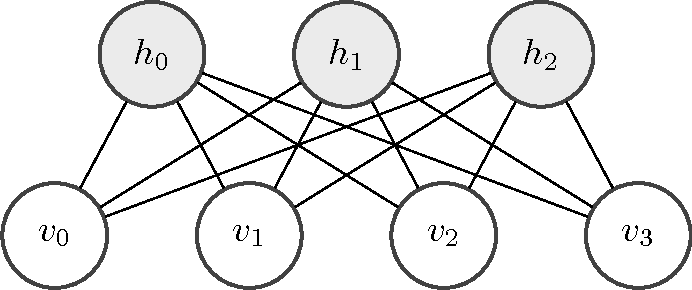
\includegraphics[scale = 0.3]{RBM.png}
  \caption{Add bunch of text here..}
\end{figure}

Further, the type of RBM we will use is the Gaussian/binary version. This type of RBM takes in continuous values for the visible neurons while the hidden neurons take the values either $0$ or $1$. Lastly about our RBM, since we are not working with any dataset, thus it's a Reinforcement learning algorithm, and not a supervised one. \\\\

For the RBM, the joint probability distribution function is defined as 
\begin{align*}
	F_{rbm}(\mathbf{X},\mathbf{H}) = \frac{1}{Z} e^{-\frac{1}{T_0}E(\mathbf{X},\mathbf{H})}
\end{align*}
where $Z$ is the partition function/normalization constant given by
\begin{align*}
	Z = \int \int \frac{1}{Z} e^{-\frac{1}{T_0}E(\mathbf{x},\mathbf{h})} d\mathbf{x} d\mathbf{h}.
\end{align*}
For this project, we will set $T_0 = 1$. The function $E(\mathbf{X},\mathbf{H})$ is the energy of a configuration of nodes. What this function does is that it gives the specifics of the relation between the visible and hidden neurons. Since, we are using the Gaussian-binary RBM, our energy of a configuration of nodes is defined as, 
\begin{align*}
	E(\mathbf{X}, \mathbf{H}) = \sum_i^M \frac{(X_i - a_i)^2}{2\sigma_i^2} - \sum_j^N b_j H_j - \sum_{i,j}^{M,N} \frac{X_i w_{ij} H_j}{\sigma_i^2} 
\end{align*}
and if the term $\sigma_i = \sigma$ then
\begin{align*}
	E(\mathbf{X}, \mathbf{H})= \frac{||\mathbf{X} - \mathbf{a}||^2}{2\sigma^2} - \mathbf{b}^T \mathbf{H} - \frac{\mathbf{X}^T \mathbf{W} \mathbf{H}}{\sigma^2}.
\end{align*}
Again, the set of visible neurons is $\mathbf{X}$ and the set of hidden neurons is $\mathbf{H}$. Further, $a$ and $b$ denotes the vector of the visible and hidden biases respectively. Lastly, $\mathbf{W}$ is the matrix containing the weights which are characterizing the connection of each visible neuron to a hidden neuron. \\\\
The only thing left now for the RBM is to find a trial wave function. The marginal distribution $P(\mathbf{X})$ is what we will use to model our wave function. We have,

\begin{align*}
	F_{rbm}(\mathbf{X}) &= \sum_\mathbf{h} F_{rbm}(\mathbf{X}, \mathbf{h}) \\
				&= \frac{1}{Z}\sum_\mathbf{h} e^{-E(\mathbf{X}, \mathbf{h})}
\end{align*}
where $\mathbf{h}$ is....... This will be used to represent our wave function. We therefore get, 
\begin{align*}
\Psi (\mathbf{X}) &= P(\mathbf{X}) =  F_{rbm}(\mathbf{X})\\
&= \frac{1}{Z}\sum_{\{h_j\}} e^{-E(\mathbf{X}, \mathbf{h})} \\
&= \frac{1}{Z} \sum_{\{h_j\}} e^{-\sum_i^M \frac{(X_i - a_i)^2}{2\sigma^2} + \sum_j^N b_j h_j + \sum_{i,j}^{M,N} \frac{X_i w_{ij} h_j}{\sigma^2}} \\
&= \frac{1}{Z} e^{-\sum_i^M \frac{(X_i - a_i)^2}{2\sigma^2}} \prod_j^N \left(1 + e^{b_j + \sum_i^M \frac{X_i w_{ij}}{\sigma^2}}\right) \\
\end{align*}
where $a_i$ and $b_i$ are elements of $a$ and $b$. With this RBM, we will be able to get a good trial wave function for us to use.

\subsection{Metropolis sampling}

\subsection{Importance sampling}
The Metropolis-Hastings or Importance sampling.. 

